\section*{Appendix} 

Here are some of our results we did not use in our report, because we did not investigate them.
However, these graphs may be really interesting to investigate further.\\
\\
First, we show our results on the effect of the Happiness Rule on the total number of moves.

\begin{figure}[H]
	\centering
    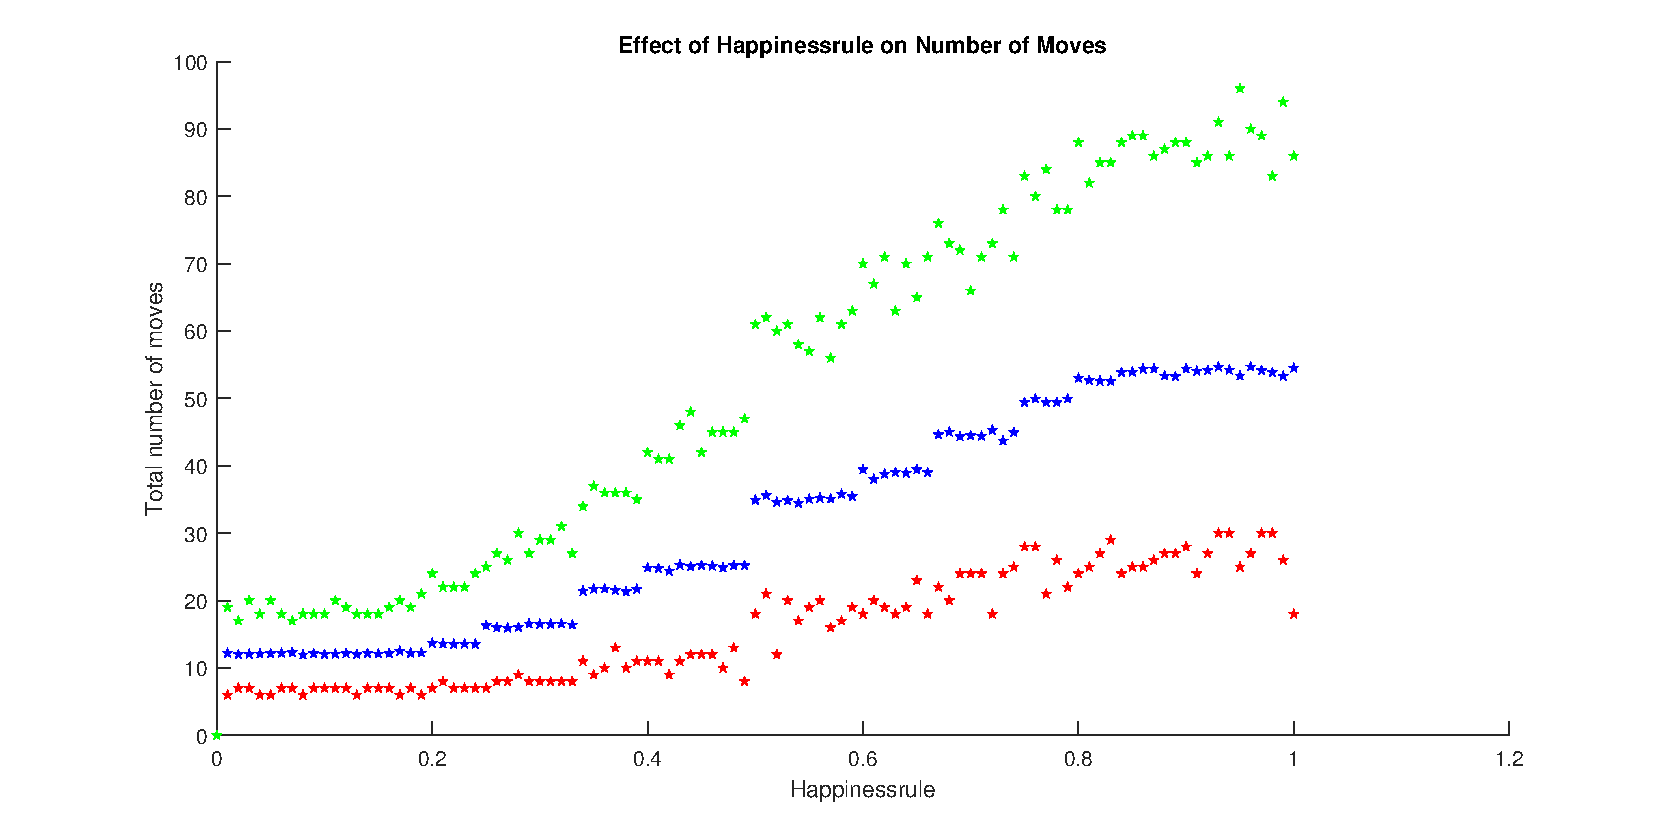
\includegraphics[width=\textwidth]{happinessregel-aantmov.pdf}
    \caption{Effect of the Happiness Rule on the total number of moves with the standard settings}
    \label{fig:happinessrule-moves}
\end{figure}

We also have some results of the effect of the random move on the number of generations.

\begin{figure}[H]
	\centering
    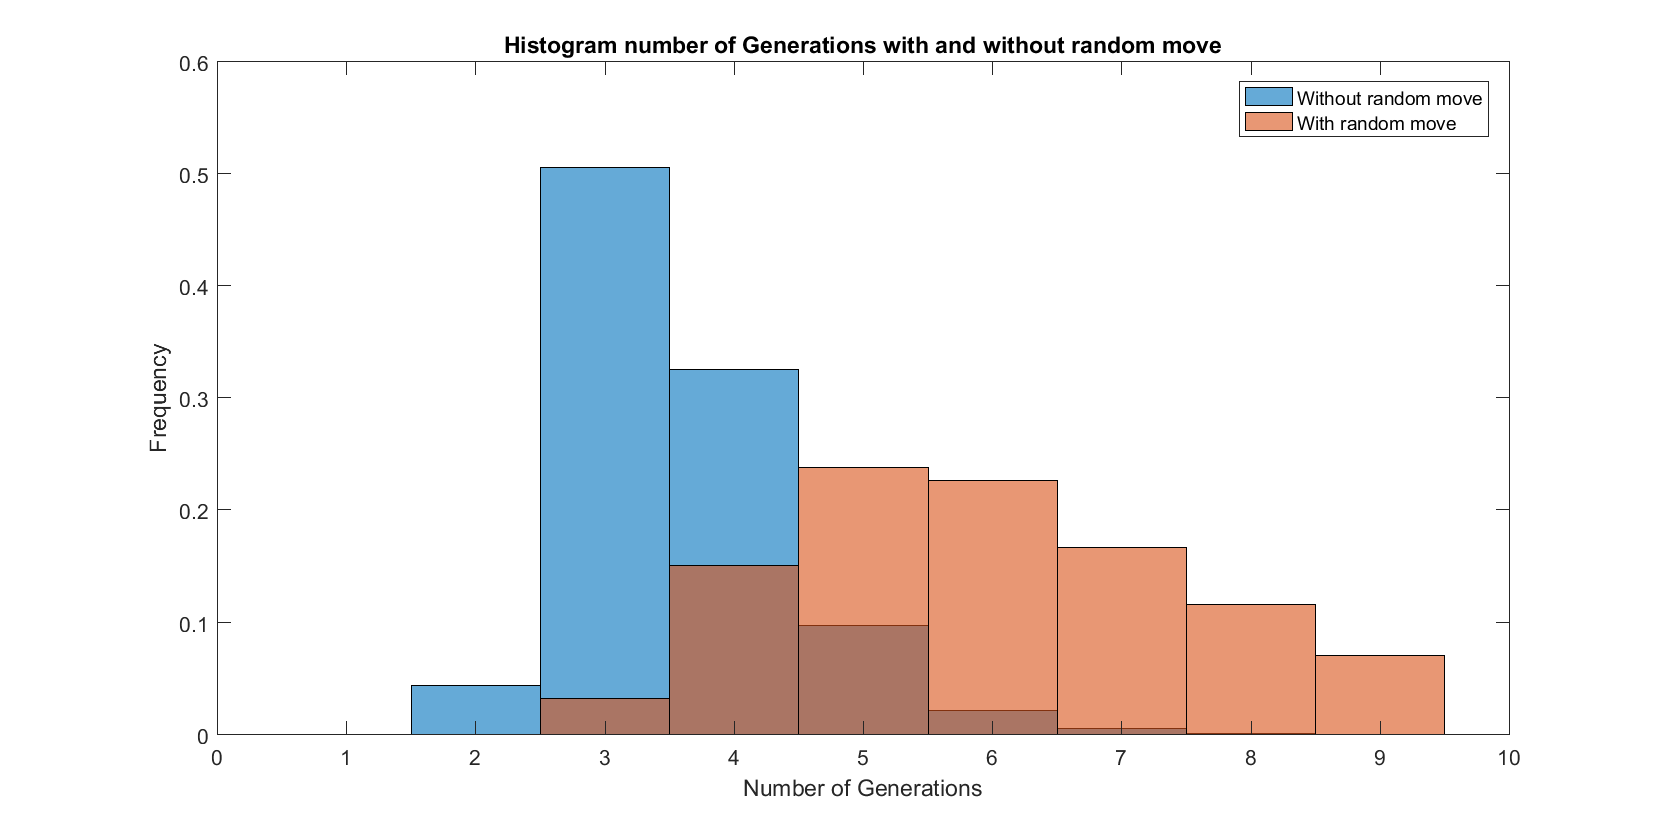
\includegraphics[width=\textwidth]{histaantgenrandverp.pdf}
    \caption{Effect of the random move on the number of generations with the standard settings}
    \label{fig:randmove-generations}
\end{figure}

Furthermore, we researched the effect of the order of neighbourhood on the number of generations, the number of moves, the segregration fraction and the average happiness of all individuals in equilibrium.

\begin{figure}[H]
	\centering
    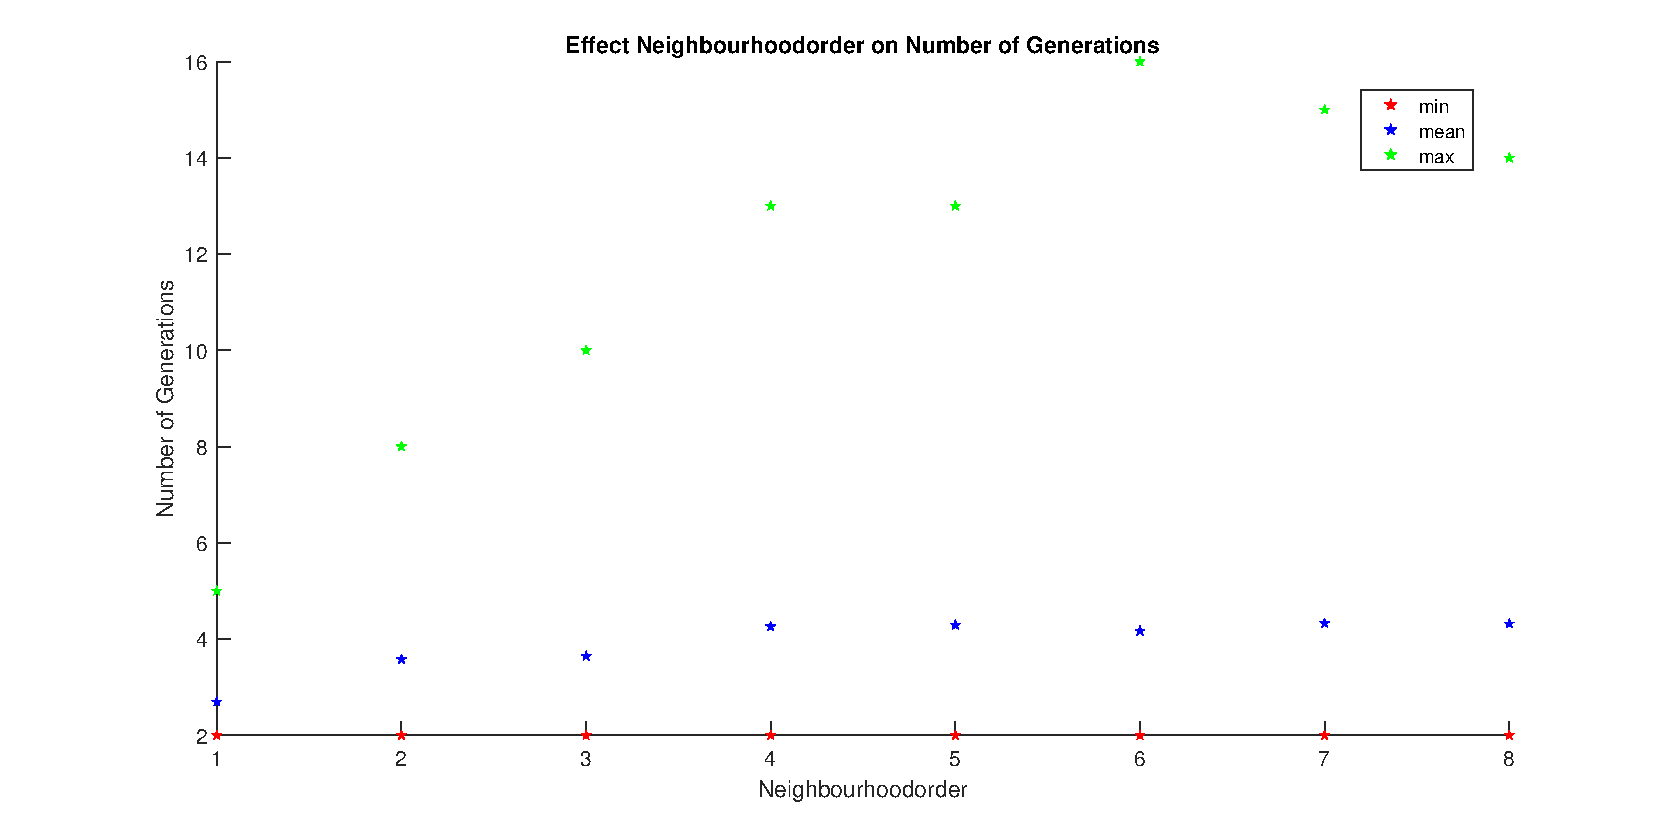
\includegraphics[width=\textwidth]{buurtorde-aantgen.pdf}
    \caption{Effect of the Neighbourhoodorder on the number of generations with the standard settings}
    \label{fig:nbho-generations}
\end{figure}

\begin{figure}[H]
	\centering
    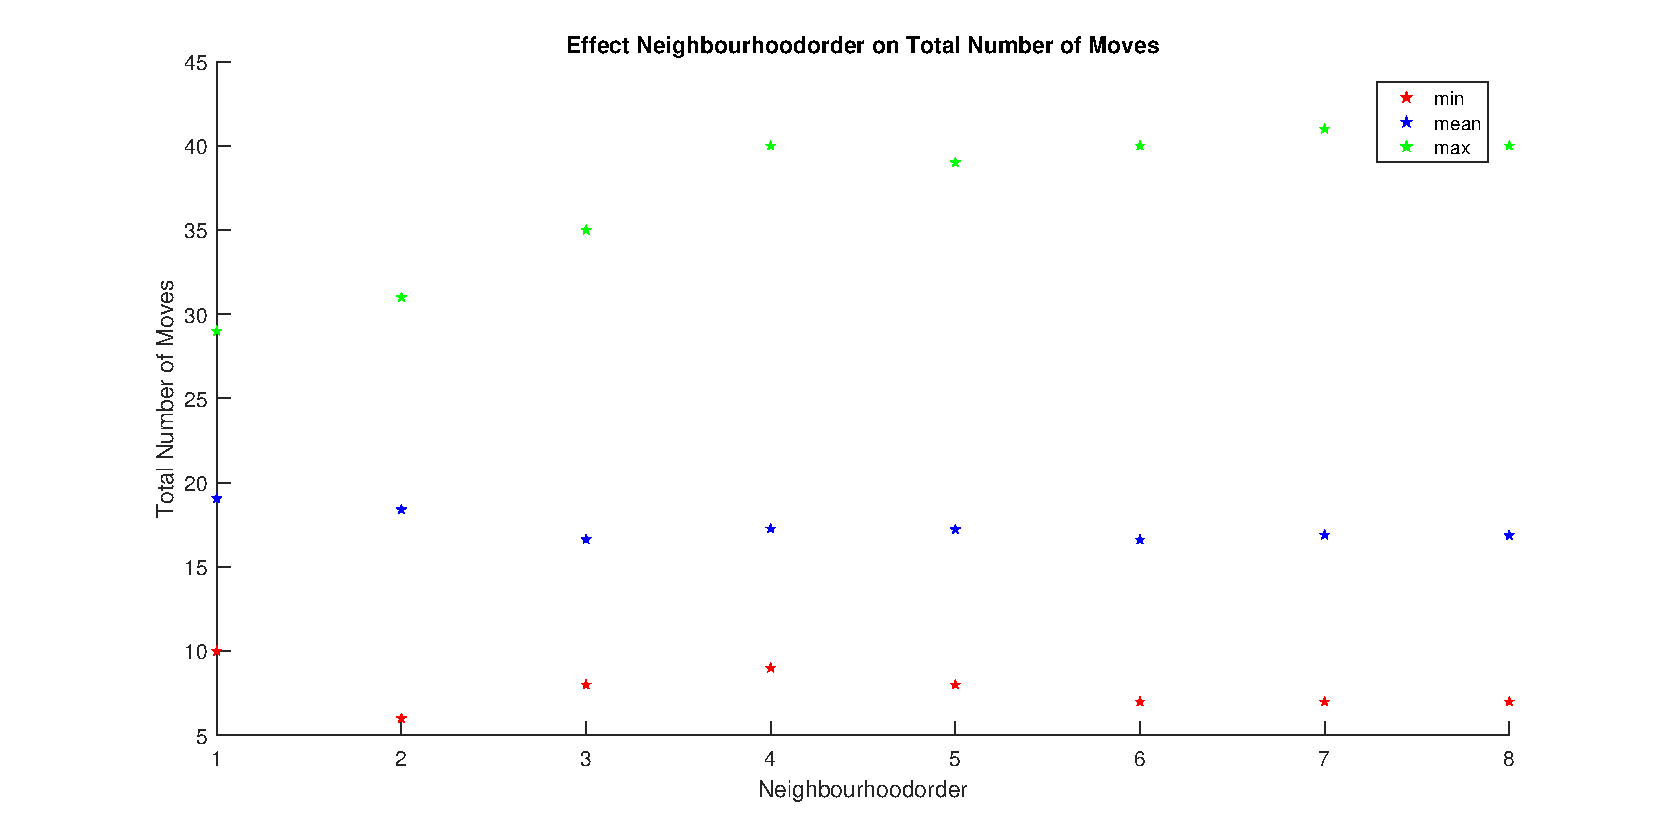
\includegraphics[width=\textwidth]{buurtorde-aantmov.pdf}
    \caption{Effect of the Neighbourhoodorder on the total number of moves with the standard settings}
    \label{fig:nbho-moves}
\end{figure}

\begin{figure}[H]
	\centering
    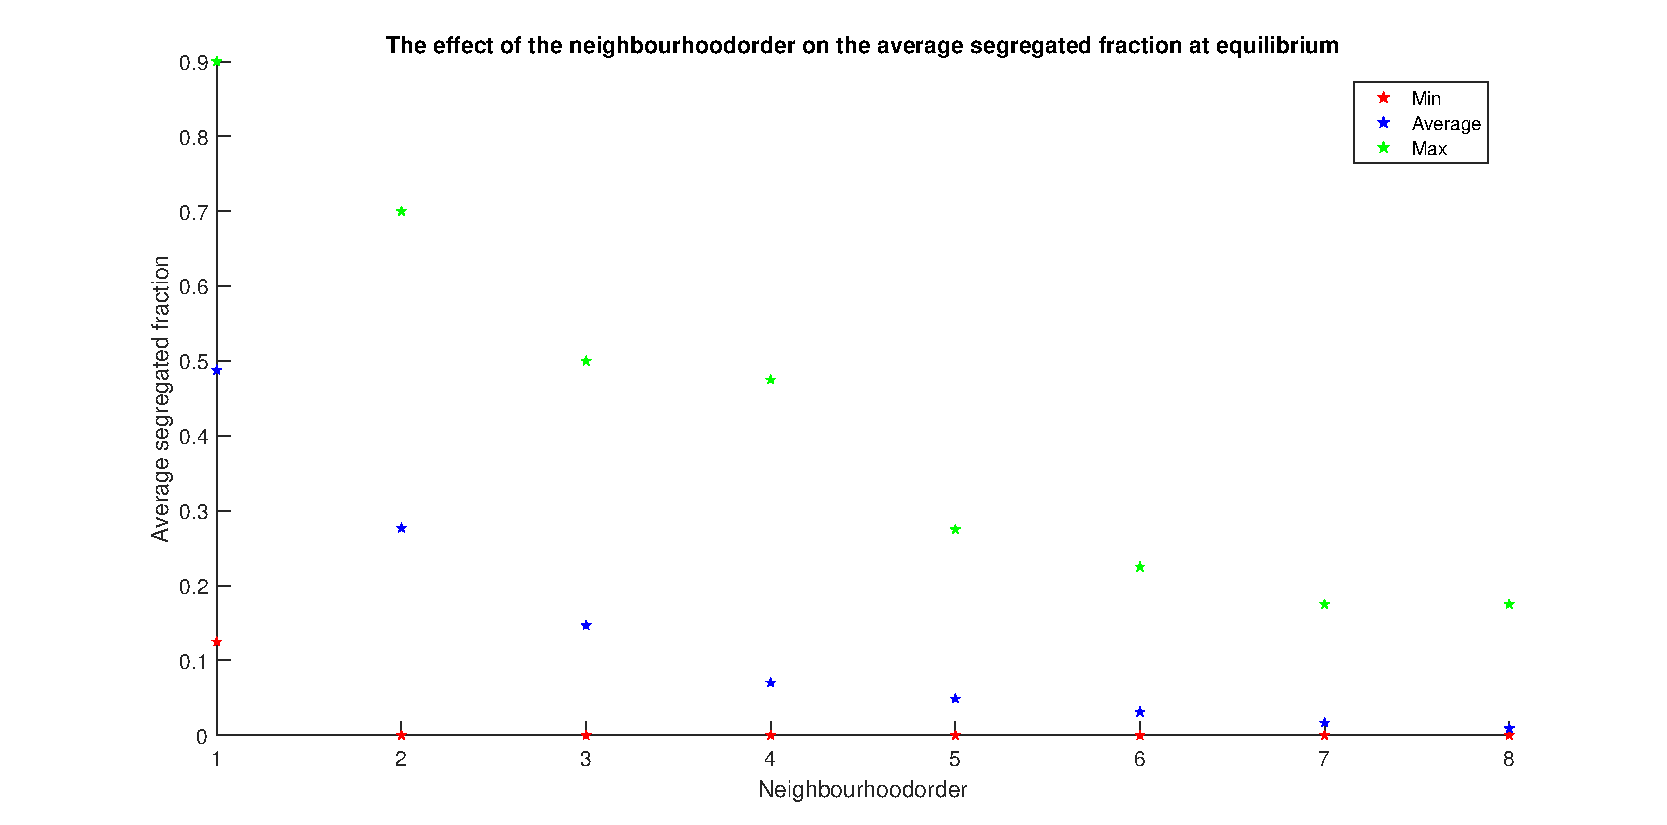
\includegraphics[width=\textwidth]{buurtorde-segreind.pdf}
    \caption{Effect of the Neighbourhoodorder on the segregated fraction in equilibrium with the standard settings}
    \label{fig:nbho-segregation}
\end{figure}

\begin{figure}[H]
	\centering
    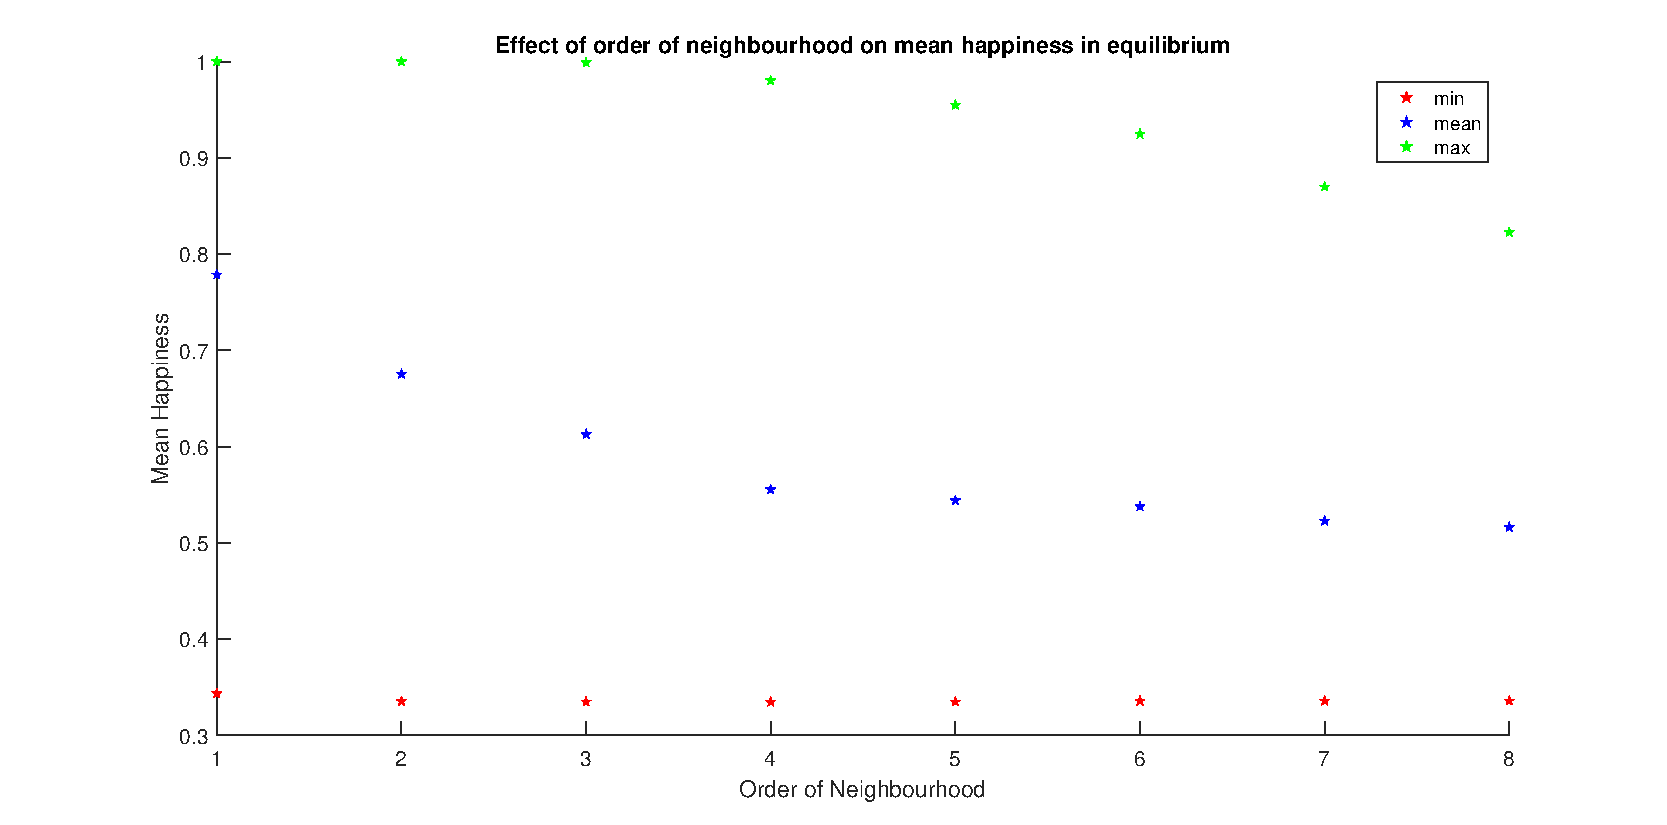
\includegraphics[width=\textwidth]{buurtorde-gemeindhappiness.pdf}
    \caption{Effect of the Neighbourhoodorder on the mean happiness in equilibrium with the standard settings}
    \label{fig:nbho-happiness}
\end{figure}

Besides, the effect of the criminals is really interesting.
Here are some effects of the number of criminals in the basic board (so the maximum number of criminals is $40$).

\begin{figure}[H]
	\centering
    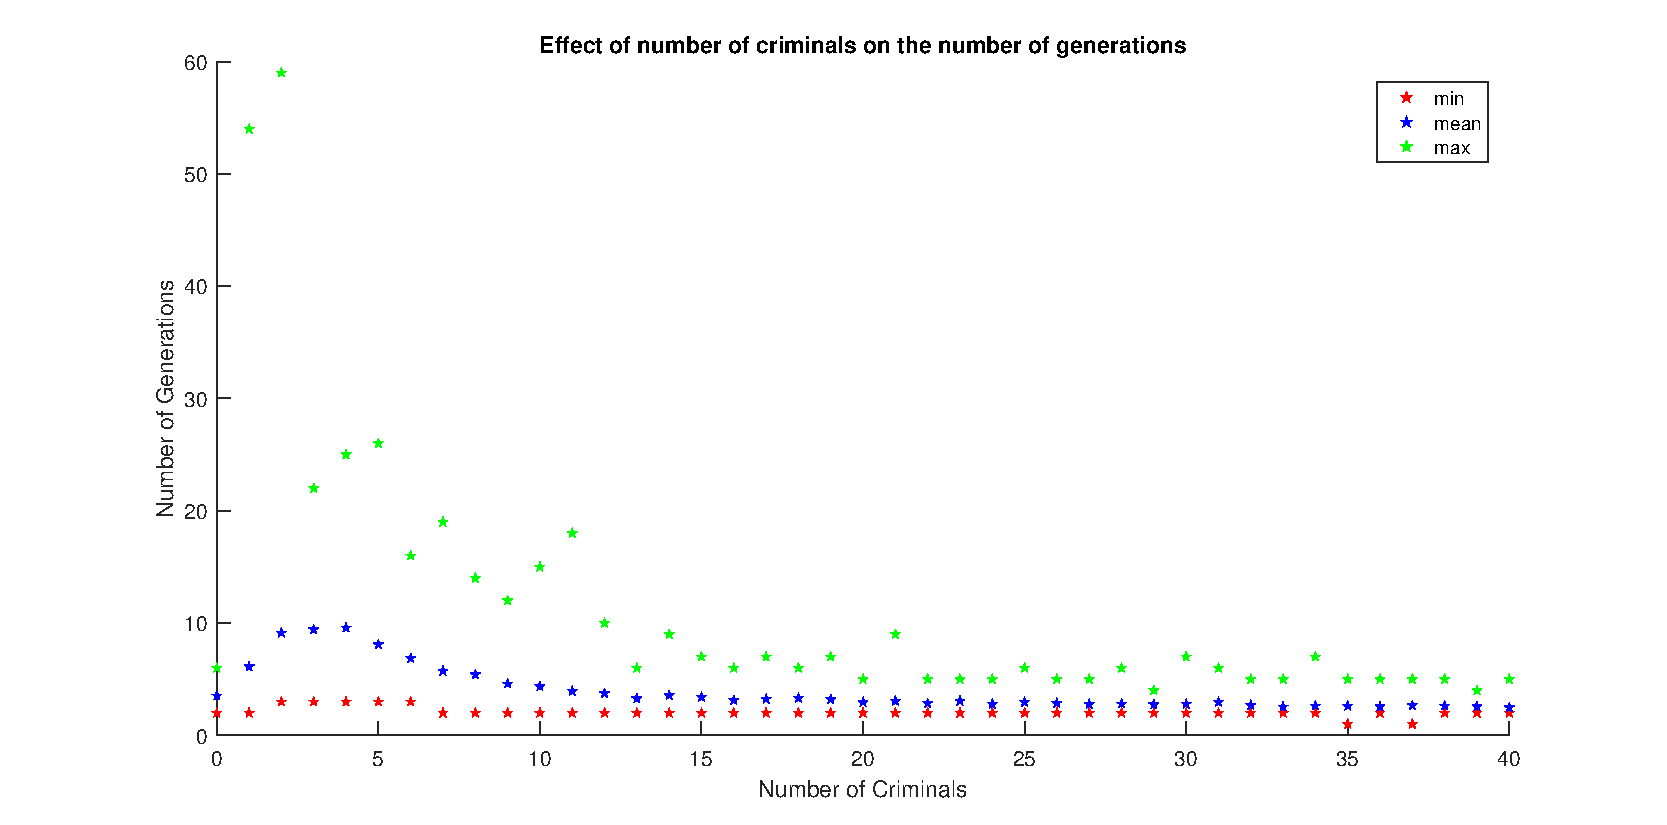
\includegraphics[width=\textwidth]{aantcrim-aantgen.pdf}
    \caption{Effect of the number of criminals on the number of generations on the basic board }
    \label{fig:cr-aantgen}
\end{figure}

\begin{figure}[H]
	\centering
    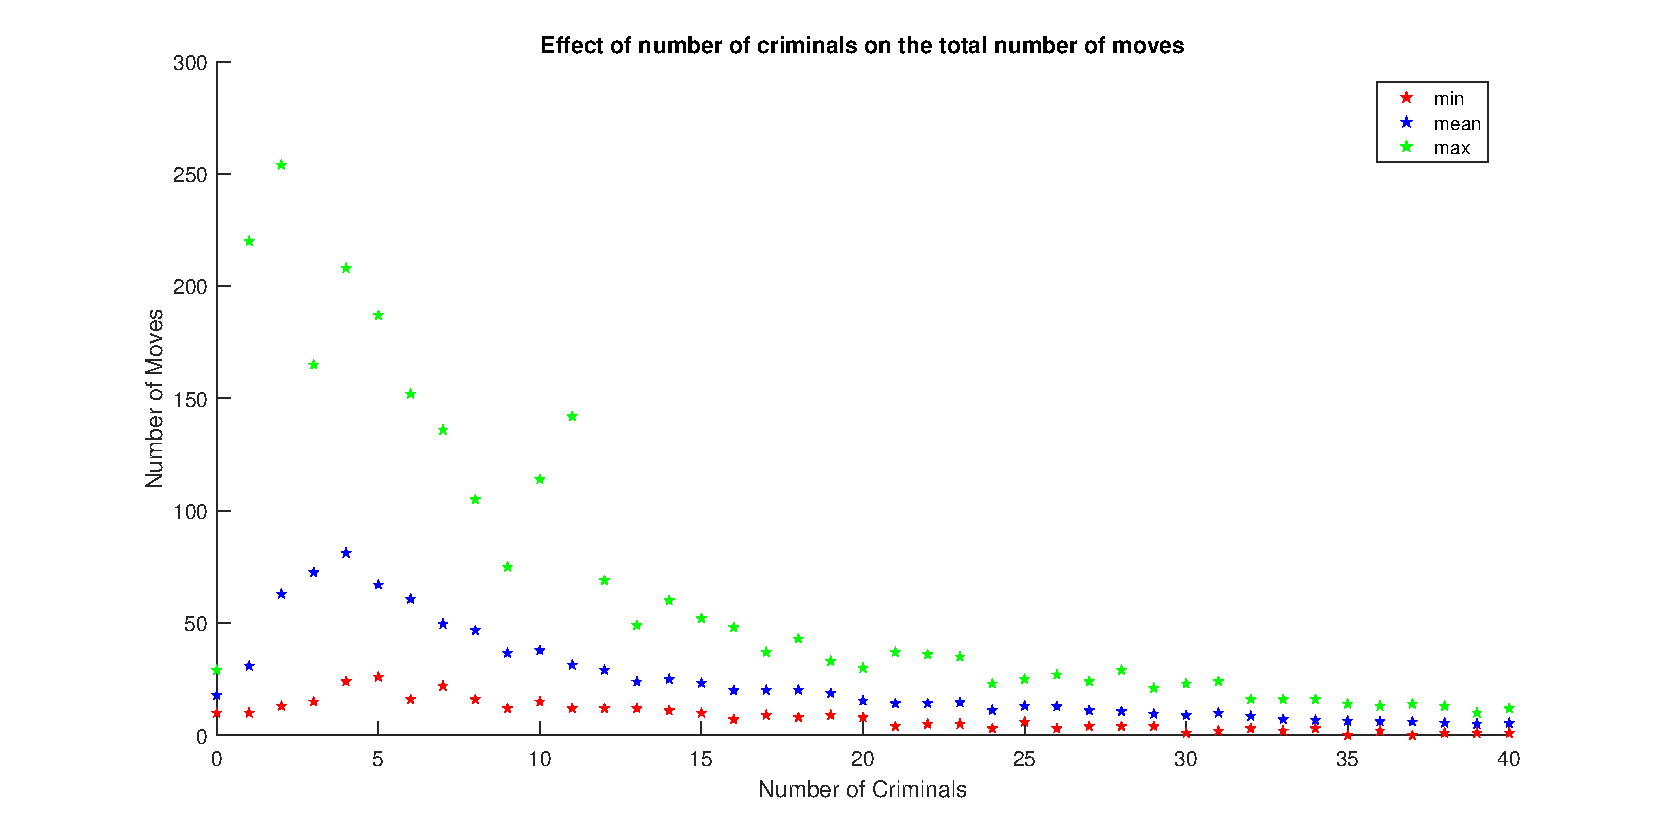
\includegraphics[width=\textwidth]{aantcrim-aantmov.pdf}
    \caption{Effect of the number of criminals on the total number of moves on the basic board}
    \label{fig:cr-aantmov}
\end{figure}

\begin{figure}[H]
	\centering
    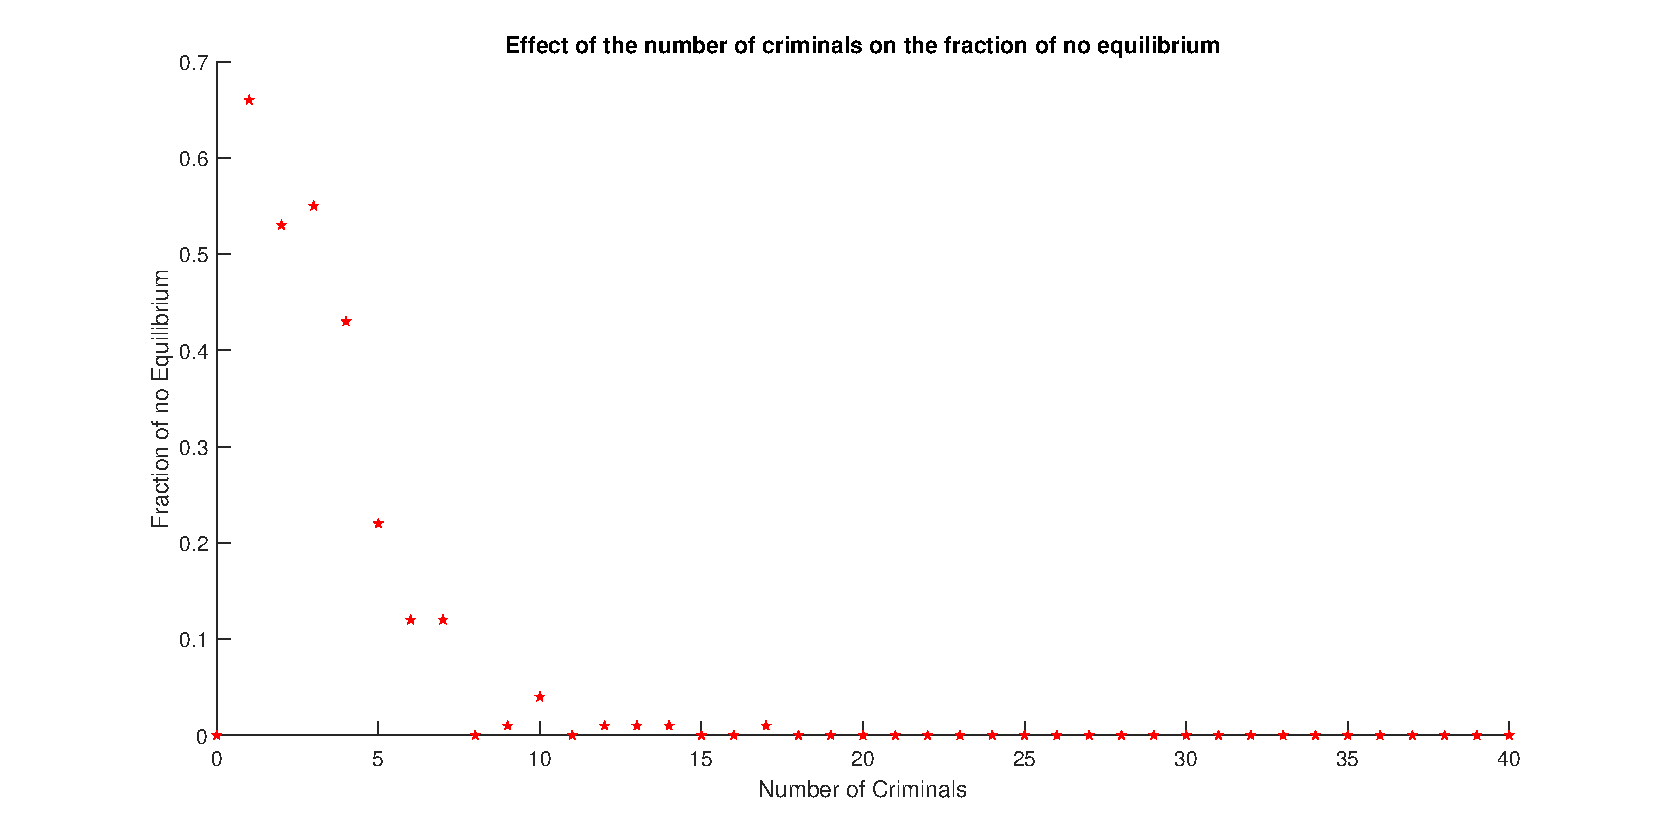
\includegraphics[width=\textwidth]{aantcrim-fracnoeq.pdf}
    \caption{Effect of the number of criminals on the relative number of times with no equilibrium on the basic board}
    \label{fig:cr-noeq}
\end{figure}

\begin{figure}[H]
	\centering
    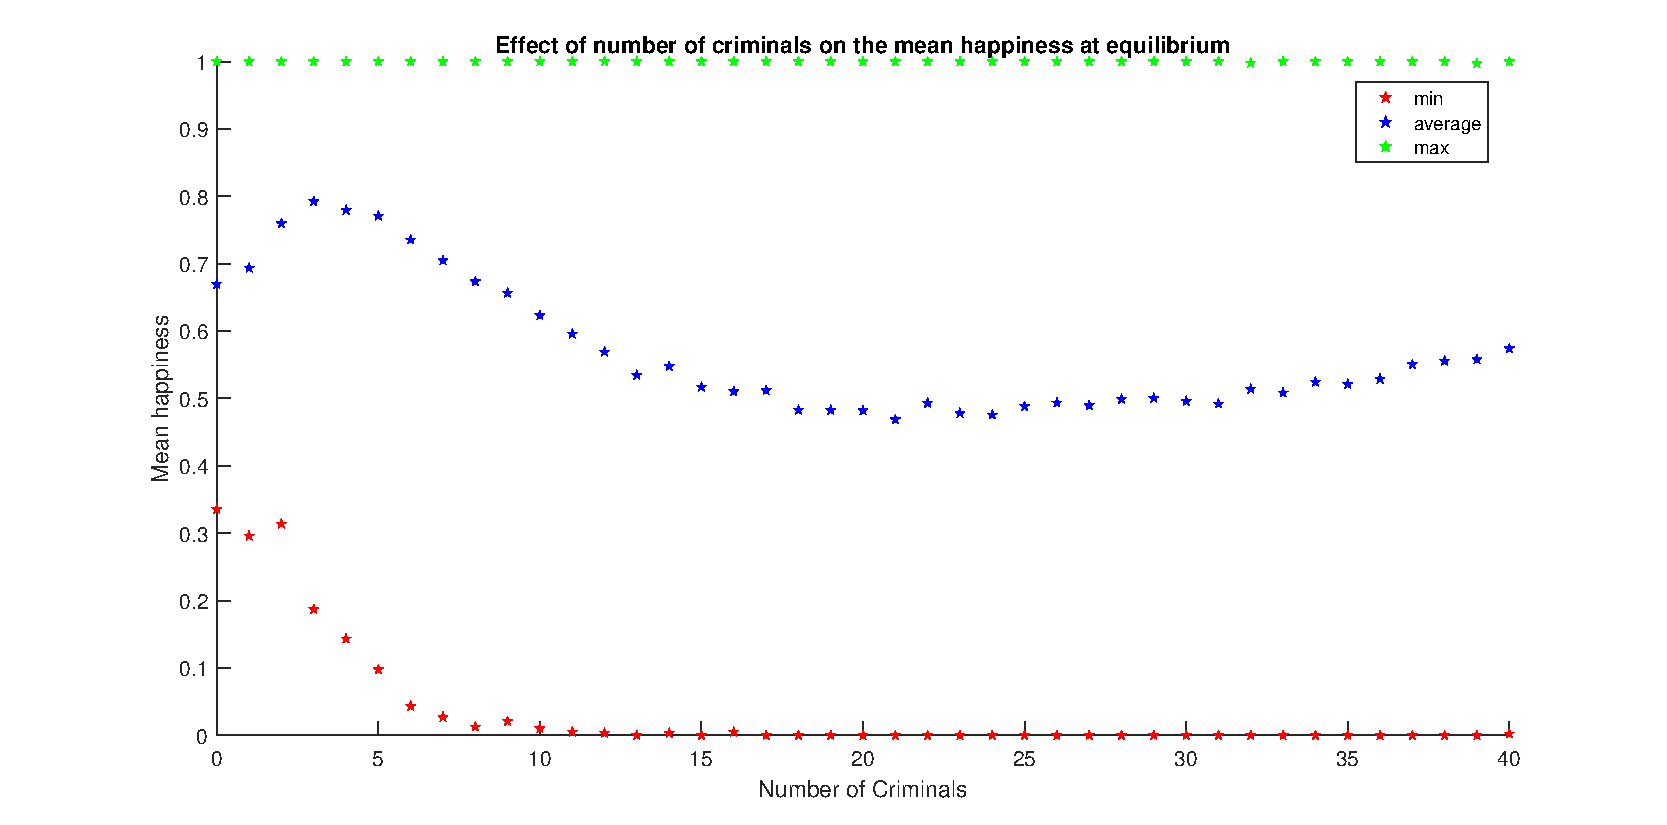
\includegraphics[width=\textwidth]{aantcrim-gemeindhappiness.pdf}
    \caption{Effect of the number of criminals on the mean happiness at equilibrium on the basic board}
    \label{fig:cr-happ}
\end{figure}

\begin{figure}[H]
	\centering
    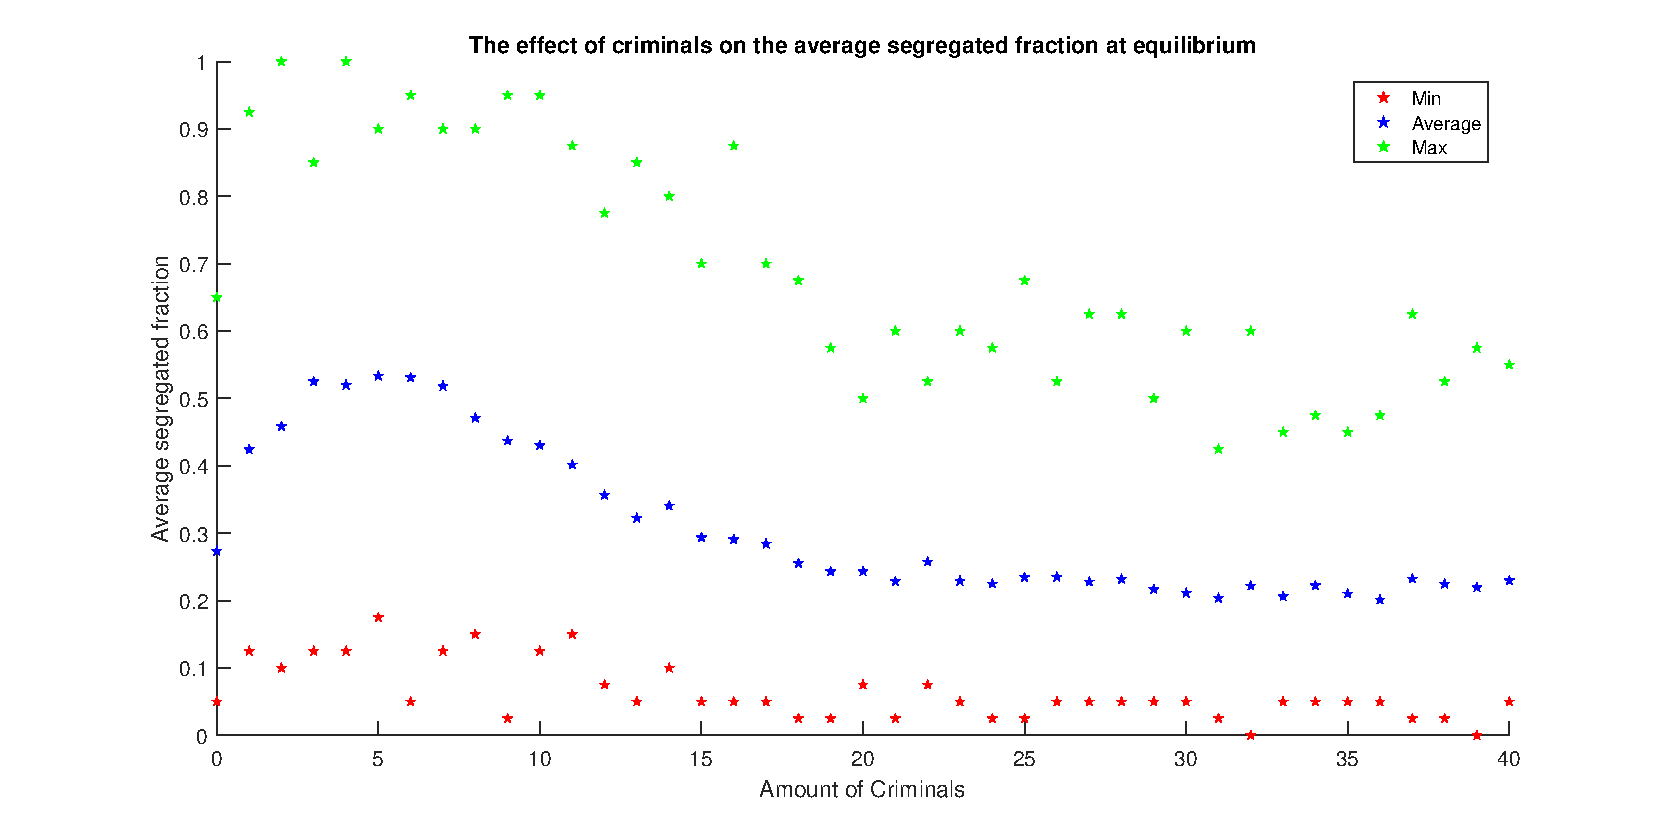
\includegraphics[width=\textwidth]{aantcrim-segreind.pdf}
    \caption{Effect of the number of criminals on the mean segregation on the basic board}
    \label{fig:cr-segr}
\end{figure}

